\chapter{The Original Uncanny Valley}
The uncanny valley was first hypothesized by Masahiro Mori, a robotics professor at the
Tokyo Institute of Technology. In an essay, published in 1970, he theorised that as the appearance of a robot 
is approaching, but failing to attain, a lifelike appearance the empathy of a person towards the robot would 
abruptly shift from affinity to revulsion.\\
At first, little attention was paid to his work however as technology evolved and more and more human-like robots were being
built the effects of the uncanny valley has gained more significance in robotics and other scientific fields. 
This paper is going to mainly focus on the effects of the uncanny valley in relation to human-robot interaction. \cite{6213238}

\section{The Uncanny Valley in Terms of Appearance}
To explain the uncanny valley in more detail Masahiro Mori chose three different robots with varying human likeness in regards to their appearance and described our feeling towards these robots. First he looked at an industrial robot which design is solely base on functionality. Given their non-existent resemblance to humans and their exclusively functional existence people feel hardly any affinity for them.\\
Next a toy robot with a roughly human looking external form was considered. Especially children can get very attached to such toys from which we can see that our affection for robots rises with a higher human resemblance.\\
To now show that the affinity for a robot does not increase linearly with its human similarity, Masahiro Mori explained that a prosthetic hand has achieved a near perfect resemblance to the human form. But as soon as a person realizes that the hand is actually artificial most people experience an eerie sensation. The loss of affinity towards the hand can be described as the uncanny valley.
In the following graph \ref{fig:uv_appearance} where the x axis corresponds to the human likeness and the y axis corresponds to the affinity all three examples are plotted to depict the uncanny valley. 
\begin{wrapfigure}{r}{0.5\textwidth} %this figure will be at the right
    \centering
    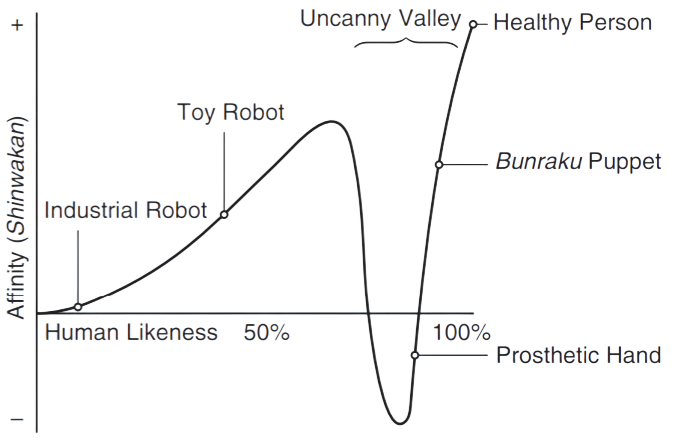
\includegraphics[width=0.5\textwidth]{graphics/uv_appearance.png}
    \caption{The uncanny valley in terms of appearance.}
    \label{fig:uv_appearance}
\end{wrapfigure}
The graph illustrates how the human likeness at first grows linearly with affinity, but at a very high but not perfect human resemblance the affinity falls rapidly.\\ Overcoming the uncanny valley is however possible according to the hyphothesis from Masahiro Mori as seen by the Banraku Puppet entry in the graph. A Bunraku is a traditional Japanese form of musical puppet theater and even though it might not be more human like than a prosthetic, on close inspection, it's total appearance and movement from a distance in a theater is very human like. Although they are very human-like they are not repulsive to the audience. \cite{6213238}

\section{The Effect of Movement}
Movement has a profound impact on the uncanny valley by amplifying the peaks and valleys seen in figure \ref{fig:uv_appearance}. This phenomenon can again be better illustrated with the example of the industrial robot and the prosthetic hand. When the industrial robot is programmed to move like a human it feels more human like and we feel a higher affinity towards the robot. On the contrary when the prosthetic hand, which already creates a strong uncanny valley effect with its appearance, starts to move the feeling of eeriness intensifies.
The figure \ref{fig:uv_movement} illustrates how adding movement steepens the slopes of the uncanny valley. \cite{6213238}\\
\begin{wrapfigure}{r}{0.5\textwidth} %this figure will be at the right
    \centering
    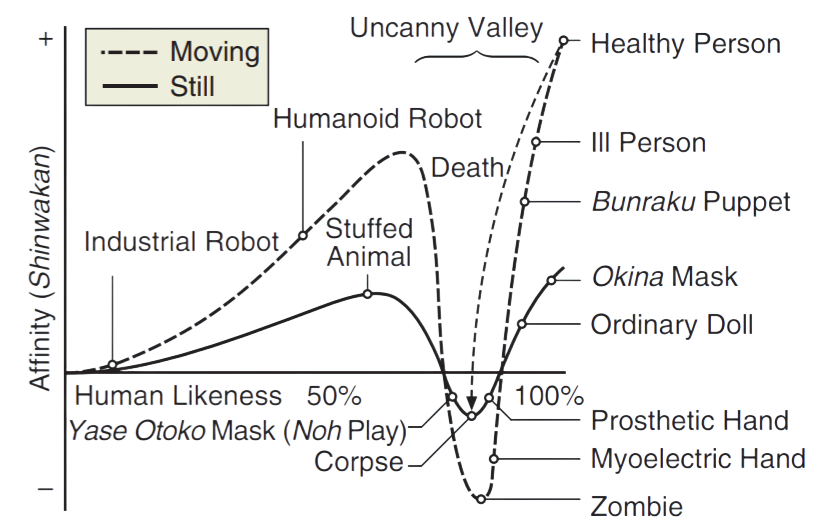
\includegraphics[width=0.5\textwidth]{graphics/uv_movement.png}
    \caption{The effect of movement on the uncanny valley.}
    \label{fig:uv_movement}
\end{wrapfigure}
Since even the movement of a single body part can have a negative effect, the unnatural movement of an entire robot can have a strong adverse effect on the affinity of the robot. Furthermore, it is very easy for a human to recognise the smallest variations in movements, which do not exactly match the human version of this movement. This can very quickly lead to an entity which has come close to an human appearance to fall deep back into the uncanny valley again. In summary, movement can amplify or even trigger the uncanny valley. \cite{6213238}
